
\documentclass[border=10pt, 12pt]{standalone}
\usepackage[svgnames]{xcolor}
\usepackage{amsmath}
\usepackage{pgfplots}
\pgfplotsset{compat=newest}
\usepackage[sfdefault]{FiraSans}
\usepackage{FiraMono}
\renewcommand*\familydefault{\sfdefault}
\begin{document}
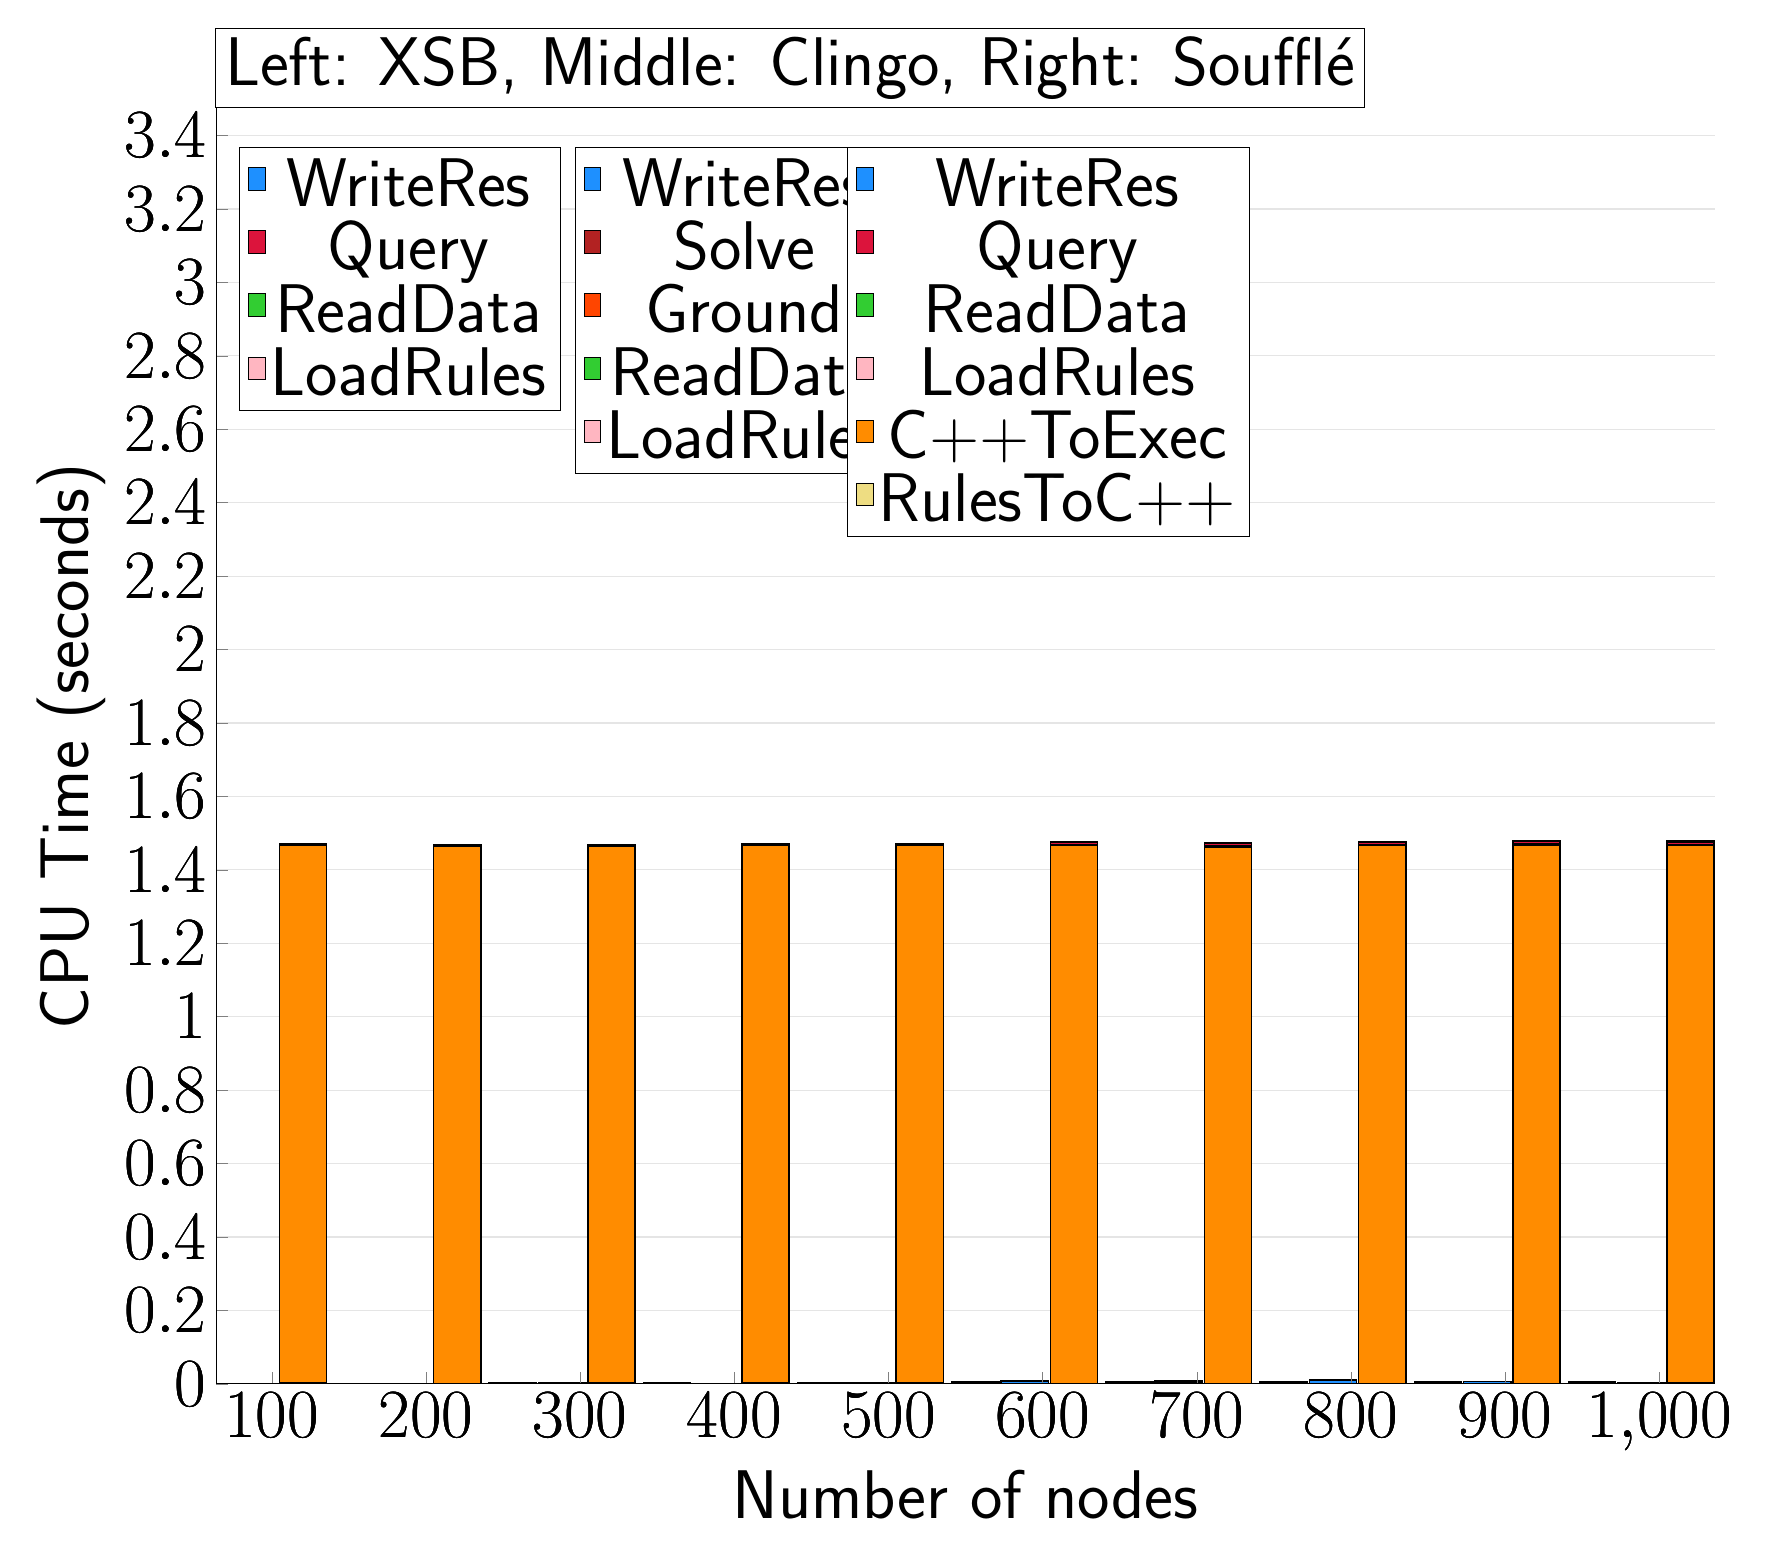
\begin{tikzpicture}
                        \begin{axis}[bar shift=-24.3pt, 
   ybar stacked,
   width=1.7\textwidth,
   bar width=0.6cm,
   ymajorgrids, tick align=inside,
   major grid style={draw=gray!20},
   xtick=data,
   ymin=0, ymax=3.4739999999999998,
   axis x line*=bottom,
   axis y line*=left,
   enlarge x limits=0.04,
   legend style={
       at={(0.23, 0.97)},
       anchor=north east,
       legend columns=1,
       font=\Huge,
   },
   ylabel={CPU Time (seconds)},
   xlabel={Number of nodes},
   label style={font=\Huge},
   tick label style={font=\Huge},
]
\addlegendimage{fill=DodgerBlue, draw=black, line width=0.2pt}
\addlegendentry{WriteRes}
\addlegendimage{fill=Crimson, draw=black, line width=0.2pt}
\addlegendentry{Query}
\addlegendimage{fill=LimeGreen, draw=black, line width=0.2pt}
\addlegendentry{ReadData}
\addlegendimage{fill=LightPink, draw=black, line width=0.2pt}
\addlegendentry{LoadRules}
\addplot +[fill=LightPink, draw=black, line width=0.55pt] coordinates {
(100, 0.0005594000000000003)
(200, 0.0005519999999999995)
(300, 0.0005565999999999995)
(400, 0.0005484000000000002)
(500, 0.0005575999999999995)
(600, 0.0005519999999999998)
(700, 0.0005548)
(800, 0.0005568)
(900, 0.0005566000000000006)
(1000, 0.0005512000000000002)
};
\addplot +[fill=LimeGreen, draw=black, line width=0.55pt] coordinates {
(100, 0.0001728000000000002)
(200, 0.0002232000000000006)
(300, 0.0003250000000000002)
(400, 0.00031899999999999984)
(500, 0.00032400000000000104)
(600, 0.0005245999999999998)
(700, 0.0005218)
(800, 0.0005182000000000002)
(900, 0.0005183999999999994)
(1000, 0.0005323999999999994)
};
\addplot +[fill=Crimson, draw=black, line width=0.55pt] coordinates {
(100, 3.259999999999998e-05)
(200, 6.159999999999986e-05)
(300, 0.00013320000000000042)
(400, 0.0001289999999999996)
(500, 0.0001339999999999994)
(600, 0.000291800000000001)
(700, 0.00028440000000000003)
(800, 0.0002819999999999996)
(900, 0.00029160000000000064)
(1000, 0.0002980000000000008)
};
\addplot +[fill=DodgerBlue, draw=black, line width=0.55pt] coordinates {
(100, 0.00027280000000000023)
(200, 0.0005932000000000003)
(300, 0.0013193999999999994)
(400, 0.0013376000000000004)
(500, 0.0013130000000000006)
(600, 0.002993599999999999)
(700, 0.0029736000000000007)
(800, 0.0029914000000000004)
(900, 0.0030071999999999994)
(1000, 0.002954799999999999)
};
\end{axis}

\begin{axis}[bar shift=-6.5pt, 
   ybar stacked,
   width=1.7\textwidth,
   bar width=0.6cm,
   ymajorgrids, tick align=inside,
   major grid style={draw=none},
   xtick=data,
   ymin=0, ymax=3.4739999999999998,
   axis x line*=none,
   axis y line*=none,
   enlarge x limits=0.04,
   legend style={
       at={(0.454, 0.97)},
       anchor=north east,
       legend columns=1,
       font=\Huge,
   },
   label style={font=\Huge},
   tick label style={font=\Huge},
]
\addlegendimage{fill=DodgerBlue, draw=black, line width=0.2pt}
\addlegendentry{WriteRes}
\addlegendimage{fill=FireBrick, draw=black, line width=0.2pt}
\addlegendentry{Solve}
\addlegendimage{fill=OrangeRed, draw=black, line width=0.2pt}
\addlegendentry{Ground}
\addlegendimage{fill=LimeGreen, draw=black, line width=0.2pt}
\addlegendentry{ReadData}
\addlegendimage{fill=LightPink, draw=black, line width=0.2pt}
\addlegendentry{LoadRules}
\addplot +[fill=LightPink, draw=black, line width=0.55pt] coordinates {
(100, 0.0)
(200, 0.0)
(300, 0.0)
(400, 0.0)
(500, 0.0)
(600, 0.0)
(700, 0.0)
(800, 0.0)
(900, 0.0)
(1000, 0.0)
};
\addplot +[fill=LimeGreen, draw=black, line width=0.55pt] coordinates {
(100, 0.0)
(200, 0.0)
(300, 0.0)
(400, 0.0)
(500, 0.0)
(600, 0.0)
(700, 0.0)
(800, 0.0)
(900, 0.0)
(1000, 0.0)
};
\addplot +[fill=OrangeRed, draw=black, line width=0.55pt] coordinates {
(100, 0.0)
(200, 0.0)
(300, 0.0)
(400, 0.0)
(500, 0.0)
(600, 0.0)
(700, 0.0020000000000000018)
(800, 0.0)
(900, 0.0)
(1000, 0.0)
};
\addplot +[fill=FireBrick, draw=black, line width=0.55pt] coordinates {
(100, 0.0)
(200, 0.0)
(300, 0.0)
(400, 0.0)
(500, 0.0)
(600, 0.0)
(700, 0.0)
(800, 0.0)
(900, 0.0)
(1000, 0.0)
};
\addplot +[fill=DodgerBlue, draw=black, line width=0.55pt] coordinates {
(100, 0.0)
(200, 0.0)
(300, 0.0020000000000000018)
(400, 0.0)
(500, 0.0020000000000000018)
(600, 0.008000000000000007)
(700, 0.006000000000000005)
(800, 0.010000000000000009)
(900, 0.006000000000000005)
(1000, 0.0020000000000000018)
};
\end{axis}

\begin{axis}[bar shift=11.3pt, 
   ybar stacked,
   width=1.7\textwidth,
   bar width=0.6cm,
   ymajorgrids, tick align=inside,
   major grid style={draw=none},
   xtick=data,
   ymin=0, ymax=3.4739999999999998,
   axis x line*=none,
   axis y line*=none,
   enlarge x limits=0.04,
   legend style={
       at={(0.69, 0.97)},
       anchor=north east,
       legend columns=1,
       font=\Huge,
   },
   label style={font=\Huge},
   tick label style={font=\Huge},
]
\addlegendimage{fill=DodgerBlue, draw=black, line width=0.2pt}
\addlegendentry{WriteRes}
\addlegendimage{fill=Crimson, draw=black, line width=0.2pt}
\addlegendentry{Query}
\addlegendimage{fill=LimeGreen, draw=black, line width=0.2pt}
\addlegendentry{ReadData}
\addlegendimage{fill=LightPink, draw=black, line width=0.2pt}
\addlegendentry{LoadRules}
\addlegendimage{fill=DarkOrange, draw=black, line width=0.2pt}
\addlegendentry{C++ToExec}
\addlegendimage{fill=LightGoldenrod, draw=black, line width=0.2pt}
\addlegendentry{RulesToC++}
\addplot +[fill=LightGoldenrod, draw=black, line width=0.55pt] coordinates {
(100, 0.0020000000000000005)
(200, 0.0)
(300, 0.0020000000000000005)
(400, 0.0020000000000000005)
(500, 0.0020000000000000005)
(600, 0.0)
(700, 0.0)
(800, 0.0)
(900, 0.0)
(1000, 0.004000000000000001)
};
\addplot +[fill=DarkOrange, draw=black, line width=0.55pt] coordinates {
(100, 1.4659999999999997)
(200, 1.464)
(300, 1.462)
(400, 1.464)
(500, 1.464)
(600, 1.466)
(700, 1.462)
(800, 1.4659999999999997)
(900, 1.4679999999999997)
(1000, 1.462)
};
\addplot +[fill=LightPink, draw=black, line width=0.55pt] coordinates {
(100, 0.0001524)
(200, 0.00015580000000000002)
(300, 9.600000000000002e-05)
(400, 0.00015299999999999998)
(500, 0.0001732)
(600, 0.0001496)
(700, 0.000148)
(800, 0.0001472)
(900, 0.0001712)
(1000, 0.000151)
};
\addplot +[fill=LimeGreen, draw=black, line width=0.55pt] coordinates {
(100, 0.0007302000000000001)
(200, 0.0009858)
(300, 0.001132)
(400, 0.0014435999999999997)
(500, 0.001414)
(600, 0.0024926)
(700, 0.002358)
(800, 0.0024056)
(900, 0.002499)
(1000, 0.0024506)
};
\addplot +[fill=Crimson, draw=black, line width=0.55pt] coordinates {
(100, 0.0006138000000000001)
(200, 0.0014373999999999997)
(300, 0.0027300000000000002)
(400, 0.0033352)
(500, 0.0031442000000000006)
(600, 0.006537800000000001)
(700, 0.0071958)
(800, 0.0065065999999999995)
(900, 0.0072896)
(1000, 0.0071182)
};
\addplot +[fill=DodgerBlue, draw=black, line width=0.55pt] coordinates {
(100, 0.0006732)
(200, 0.0009508000000000001)
(300, 0.0012392)
(400, 0.0014426)
(500, 0.0015065999999999999)
(600, 0.0019682000000000002)
(700, 0.0022220000000000005)
(800, 0.0021804)
(900, 0.0022823999999999995)
(1000, 0.0022734)
};
\end{axis}


\node[anchor=south, draw, fill=white] at (rel axis cs:0.42, 1) {\Huge Left: XSB, Middle: Clingo, Right: Soufflé};
\end{tikzpicture}
\end{document}
                    